
%(BEGIN_QUESTION)
% Copyright 2008, Tony R. Kuphaldt, released under the Creative Commons Attribution License (v 1.0)
% This means you may do almost anything with this work of mine, so long as you give me proper credit

Suppose a control valve with a linear inherent characteristic and a maximum flow capacity of 18 ($C_v$ = 18) is installed at the base of a dam, where it experiences a constant downstream pressure of 0 PSI (atmospheric) and an upstream pressure that varies with flow rate (owing to the pressure losses along the skinny pipe):

$$\includegraphics[width=15.5cm]{i03228x01.eps}$$

A ``load line'' for this piping system has been superimposed on the control valve's characteristic curve set.  Use this graph to determine the water flow rates at 0\% open, 25\% open, 50\% open, 75\% open, and 100\% (full) open:

$$\includegraphics[width=15.5cm]{i03228x02.eps}$$

$$\vbox{\offinterlineskip
\halign{\strut
\vrule \quad\hfil # \ \hfil & 
\vrule \quad\hfil # \ \hfil & 
\vrule \quad\hfil # \ \hfil \vrule \cr
\noalign{\hrule}
%
% First row
Opening & $C_v$ & Flow rate \cr
%
(\%) &  & (GPM) \cr
%
\noalign{\hrule}
%
% Another row
0 & 0 & \cr
%
\noalign{\hrule}
%
% Another row
25 & 4.5 & \cr
%
\noalign{\hrule}
%
% Another row
50 & 9 & \cr
%
\noalign{\hrule}
%
% Another row
75 & 13.5 & \cr
%
\noalign{\hrule}
%
% Another row
100 & 18 & \cr
%
\noalign{\hrule}
} % End of \halign 
}$$ % End of \vbox

\underbar{file i03228}
%(END_QUESTION)





%(BEGIN_ANSWER)

$$\vbox{\offinterlineskip
\halign{\strut
\vrule \quad\hfil # \ \hfil & 
\vrule \quad\hfil # \ \hfil & 
\vrule \quad\hfil # \ \hfil \vrule \cr
\noalign{\hrule}
%
% First row
Opening & $C_v$ & Flow rate \cr
%
(\%) &  & (GPM) \cr
%
\noalign{\hrule}
%
% Another row
0 & 0 & 0 \cr
%
\noalign{\hrule}
%
% Another row
25 & 4.5 & 19.4 \cr
%
\noalign{\hrule}
%
% Another row
50 & 9 & 38.1 \cr
%
\noalign{\hrule}
%
% Another row
75 & 13.5 & 53.8 \cr
%
\noalign{\hrule}
%
% Another row
100 & 18 & 67.5 \cr
%
\noalign{\hrule}
} % End of \halign 
}$$ % End of \vbox

\vskip 10pt

Follow-up question: if we were to plot a graph of flow rate ($Q$) versus valve stem opening (\%), would it be linear for this system?  Explain why or why not.

%(END_ANSWER)





%(BEGIN_NOTES)

A graph of $Q$-versus-\% opening would not be linear.  Despite the control valve's inherently linear characteristic, the pressure drop across the valve does not remain constant.

%INDEX% Electronics review: load lines
%INDEX% Final Control Elements, valve: characterization

%(END_NOTES)


